\section{Event selection and reconstruction}

In this chapter the procedure for reconstruction of the events where one $B$ meson decays inclusively
to a $\Lambda_c$ baryon and the accompanying $B$ meson decays hadronically.

\subsection{$B_{tag}$ reconstruction}

The FEI is an exclusive tagging algorithm that uses machine learning to reconstruct
$B$ meson decay chains and calculates the probability that these decay chains correctly
describe the true process. In this analysis only hadronically reconstructed decay chains are
considered. The training called \texttt{FEI\_}\texttt{B2BII\_}\texttt{light-2012-minos} is used. Tag-side $B$ meson candidates are required to have a beam-constrained mass greater than 5.22 GeV/c$^2$ and $- 0.15 < \Delta E < 0.07 $   GeV. \\
In the case of multiple candidates in the same event, the candidate with the highest SignalProbability (the signal probability calculated by FEI using FastBDT) is chosen. To suppress the background constisting of $B^0$ events misreconstructed as $B^+$ (and vice-versa) from neutral (charged) decays also a $B^0$ ($B^+$) candidate is reconstructed with FEI and if its SignalProbability is higher than the charged (neutral) reconstructed $B$ meson, the event is discarded. This constitutes a sort of crossfeed-veto, rejecting part of events belonging to the other typology of decays of interest: for example in the case one is interested in reconstructing $B^{+/-}$ decays and the event actually contains $B^0/\bar{B^0}$ decays, the FEI reconstructed neutral $B$ meson candidate most likely presents a higher SignalProbability than the charged FEI reconstructed candidate.

\subsection{$\Lambda_c$ reconstruction}

In the \textit{rest of event} (ROE) of the reconstructed $B_{tag}$ meson, to select $\Lambda_c \rightarrow p  K \pi$ signal candidates, the following event selection criteria are applied (same PID cuts were used for example in the Belle Note 1521 \url{https://belle.kek.jp/secured/belle_note/gn1521/BN_v1.pdf}). 
Charged tracks with the impact parameters perpendicular to and along the nominal interaction point (IP) are required to be less than 2 cm and 4 cm respectively ($dr <$ 2 cm and $|dz| <$ 4 cm).\\
The pion tracks are required to be identified with $\frac{\mathcal{L_{\pi}}}{\mathcal{L}_{K}+\mathcal{L_{\pi}}} > 0.6$. The kaon tracks are required to be identified with $\frac{\mathcal{L}_{K}}{\mathcal{L_{K}}+\mathcal{L_{\pi}}} > 0.6$, and the proton/anti-proton tracks are required to be identified with  
$\frac{\mathcal{L}_{p/\bar{p}}}{\mathcal{L}_{K}+\mathcal{L}_{p/\bar{p}}} > 0.6$ and $\frac{\mathcal{L}_{p/\bar{p}}}{\mathcal{L}_{\pi}+\mathcal{L}_{p/\bar{p}}} > 0.6$, where the $\mathcal{L}_{\pi ,} {}_{K,} {}_{p/\bar{p}}$ are the likelihoods for pion, kaon, proton/anti-proton, respectively, determined using the ratio of the energy deposit in the ECL to the momentum measured in the SVD and CDC, the shower shape in the ECL, the matching between the position of charged
track trajectory and the cluster position in the ECL, the hit information from the
ACC and the dE/dx information in the CDC. \\
For the $\Lambda_c$ candidates a vertex fit is performed with \texttt{TreeFitter}, requiring it to converge.  If there are more than one $\Lambda_c$ combination, then the best candidate based on the $\chi^2$ probability is chosen. The $\Lambda_c$ signal region is defined to be $|M_{\Lambda_c} - m_{\Lambda_c}| < $   20  MeV/$c^2$ ($\sim$ 3$\sigma$), here $m_{\Lambda_c}$ is the nominal mass of $m_{\Lambda_c}$.\\



\begin{figure}[H]
%\centering
{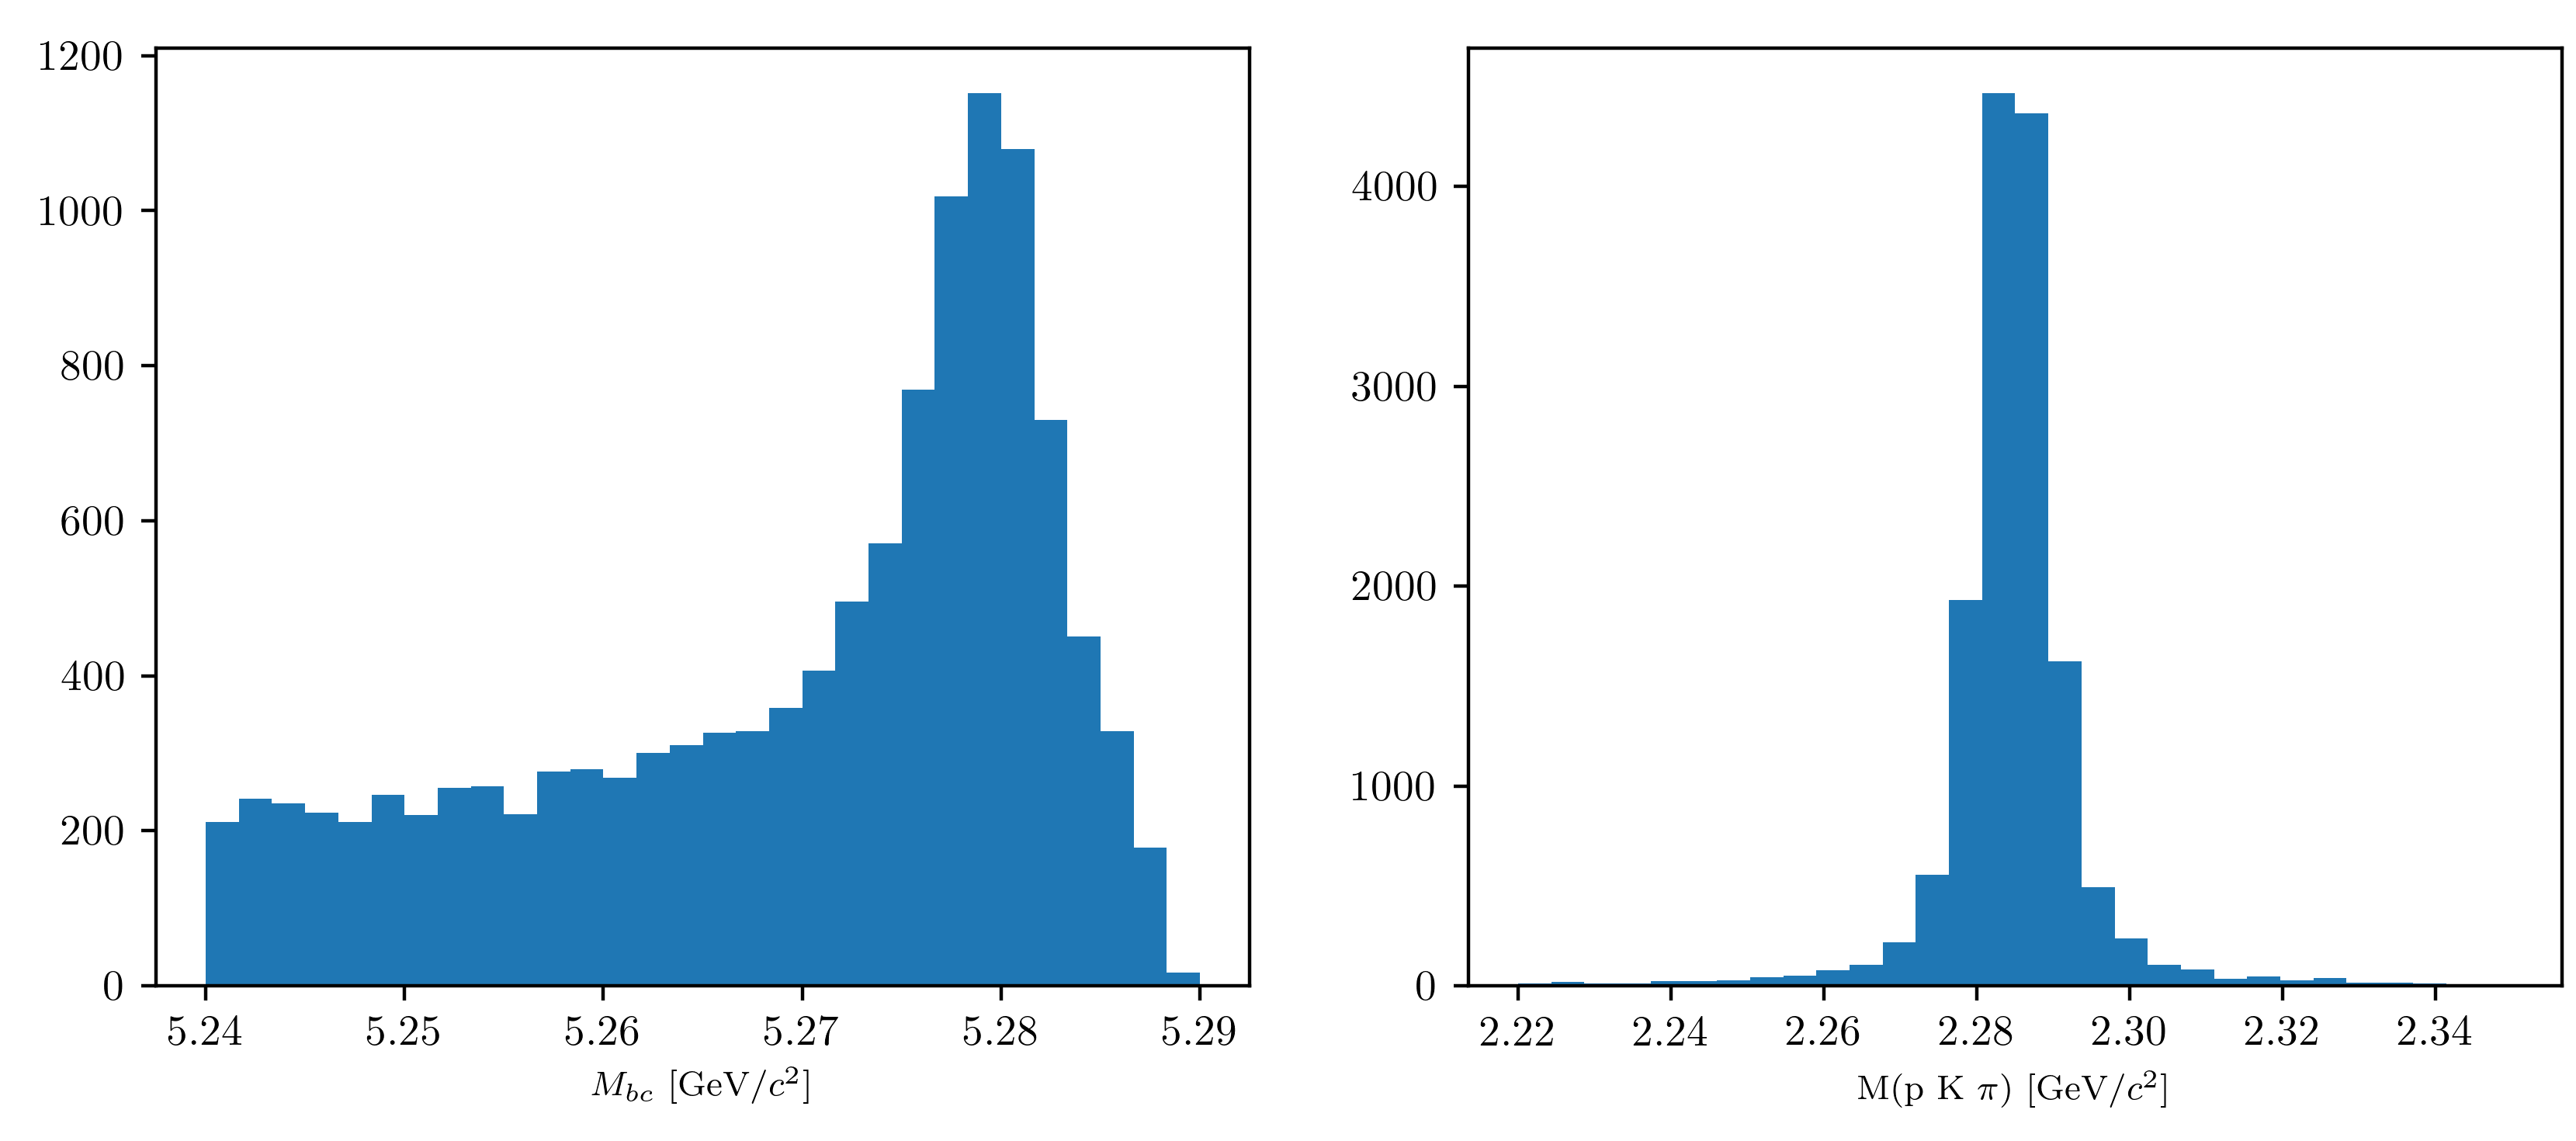
\includegraphics[width=1.0\textwidth]{03-Selection/figs/chargedBcorr_Mbc_MpKpi_TotalSignal.png}}
\caption{$M_{bc}$ and $M(p K \pi)$ distributions of $B_{tag}$ and $\Lambda_c$ candidates reconstructed in the signal sample.}
\label{fig:chargedBcorr_Mbc_MpKpi_TotalSignal}
\end{figure}

\subsection{Wrongly reconstructed $B_{tag}$ candidates}\label{wronglyBtag}

In the case of the signal sample the distributions for the beam-constrained mass $M_{bc}$ and for the correctly reconstructed $\Lambda_c$ candidates, look
like in \cref{fig:chargedBcorr_Mbc_MpKpi_TotalSignal}. If one then investigates the $M_{bc}$ distribution of the $B_{tag}$ candidates reconstructed with 
FEI, it can be seen that there is a peaking structure for wrongly reconstructed $B$ 
mesons (as in \cref{fig:wrongly_recoB}), according to the BASF2 internal truth matching variable \textbf{isSignal}.
It is obvious from this that the BASF2 internal truth matching variable cannot be used to separate properly the signal events in correctly and wrongly reconstructed $B$ mesons. In the study  BELLE2-NOTE-TE-2021-026 \url{https://docs.belle2.org/record/2711/files/BELLE2-NOTE-TE-2021-026.pdf} a possible solution was found developing new variables that can be used for an improved truth matching for the FEI (those variables were added to a newer BASF2 release than the one used for this study). In the present study instead a more "traditional" approach was adopted: fitting the $M_{bc}$ distribution with a sum of PDFs that account for the flat (background) component and the peaking (signal) component. The first component represents the combinatorial background, i.e. $B$ mesons that were mis-reconstructed, and therefore those events are denoted from now on as    "\textbf{misreconstructed signal}".  
The peaking component represents the correctly reconstructed signal events in $M_{bc}$ and therefore denoted from now on as "\textbf{reconstructed signal}".  Only the second one is then considered for the signal yield, while the first is counted as a background.
To validate this method a control decay study was performed on the flavor correlated $B^+ \rightarrow \bar{D^0}$ channel. 


\begin{figure}[h!]
\centering
{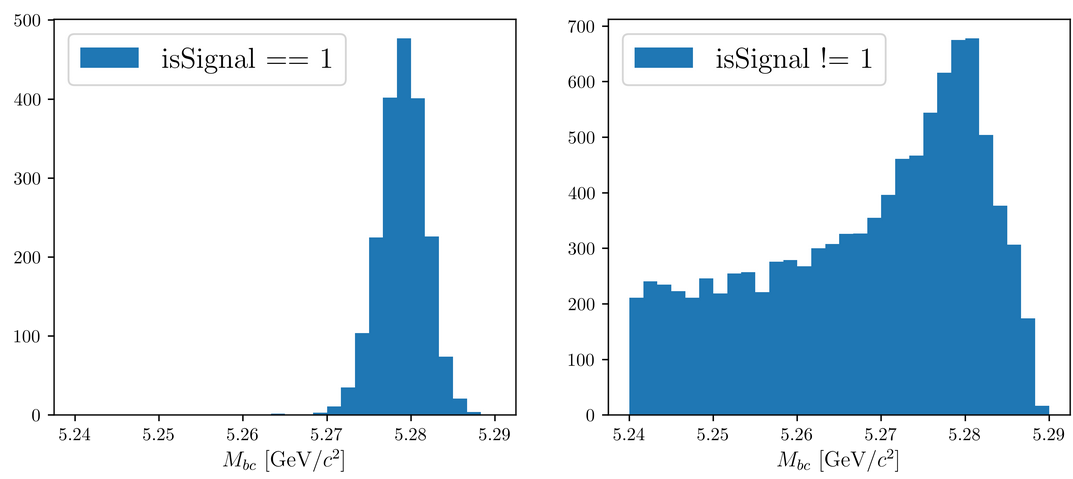
\includegraphics[width=1.\textwidth]{03-Selection/figs/wrongly_recoB.png}}
\caption{$M_{bc}$ distribution of $B_{tag}$ candidates reconstructed in the signal sample, truth-matched (on the left) and not (on the right).}
\label{fig:wrongly_recoB}
\end{figure}



\section{Signal selection optimization}

To further enhance the purity of the signal decays, an optimization procedure is adopted to determine optimal cuts for a set of variables for each decay mode under investigation by this study.
The cuts on the following variables are optimized:
\begin{itemize}
    \item $foxWolframR2$: the event based ratio
of the 2-nd to the 0-th order Fox-Wolfram moments
    \item SignalProbability: the already mentioned signal probability calculated by FEI using FastBDT
    \item $p^{\Lambda_c}_{CMS}$: momentum of the $\Lambda_c$ candidates in the center of mass system
\end{itemize}

The optimization is based on the Figure Of Merit (FOM): FOM = $\frac{S}{\sqrt{S+B}}$

Where S and B are respectively signal and background events in the signal region: $M_{bc} > $ 5.27 GeV/$c^2$,  2.2665  $< M(p K \pi) <$ 2.3065 GeV/$c^2$.\\
Due to the issue reported in Sec. \ref{wronglyBtag}, to separate signal events that peak in $M_{bc}$ from the ones that are not (which are then categorized as background events), the events reconstructed in the signal sample are fitted. with a sum of Crystal Ball function and Argus for each cut value on the corresponding variable to optimize (as in \cref{fig:wrongB_Mbc}).

\begin{figure}[h!]
%\centering
{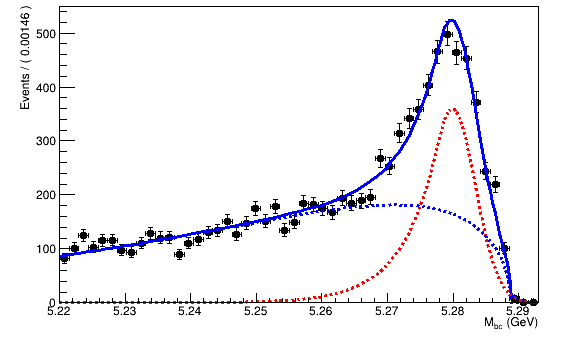
\includegraphics[width=0.75\textwidth]{03-Selection/figs/wrongB_Mbc.png}}
\caption{Example of a fit used to separate the correctly reconstructed $B$ mesons (described by the red dotted Crystal Ball function) from the wrongly reconstructed ones (described by the blue dotted Argus function).}
\label{fig:wrongB_Mbc}
\end{figure}

